\documentclass[russian, utf8, nocolumnxxxi, nocolumnxxxii, 14pt]{eskdtext}
\usepackage[utf8]{inputenc}
\usepackage[T1,T2A]{fontenc}
\usepackage[english, russian]{babel}
\usepackage[argument]{graphicx}
\usepackage{graphicx}
\graphicspath{{images/}}
\usepackage{wrapfig}
\usepackage{tikz}
\usepackage{siunitx}
\usepackage[american,cuteinductors,smartlabels]{circuitikz}
\setlength{\parskip}{0pt}
\renewcommand{\baselinestretch}{1.25}
\renewcommand{\ESKDtheTitleFieldX}{2018}

\ESKDdepartment{МИНОБРНАУКИ РОССИИ}
\ESKDcompany{
САНКТ-ПЕТЕРБУРГСКИЙ ГОСУДАРСТВЕННЫЙ \\
ЭЛЕКТРОТЕХНИЧЕСКИЙ УНИВЕРСИТЕТ\\
«ЛЭТИ» ИМ. В.И. УЛЬЯНОВА (ЛЕНИНА)\\
Кафедра робототехники и автоматизации\\ 
производственных систем}
\ESKDtitle{ПОЯСНИТЕЛЬНАЯ ЗАПИСКА К КУРСОВОЙ РАБОТЕ}
\ESKDdocName{по дисциплине "Информатика"\\
Тема: Решение математических задач с использование математических пакетов Scilab и Reduce-algebra\\
Вариант 22}
\ESKDtitleDesignedBy{Студент группы 8871}{Турыгин Д.А.}
\ESKDtitleDesignedBy{Старший преподаватель}{Прокшин А.Н.}
\ESKDauthor{Турыгин}
\ESKDchecker{Прокшин}
\ESKDcolumnI{\small Решение математических задач с использование математических пакетов Scilab и Reduce-algebra}
\ESKDcolumnII{Вариант 22}
\ESKDcolumnIVfII{У}
\ESKDcolumnIX{СПбГЭТУ гр.8871}

\begin{document}
\maketitle
\newpage
\tableofcontents
\newpage
\section{Постановка задачи курсовой работы.} \\
\indent В современных реалиях, ведение инженерной работы не обходится без сложных вычислений, осуществление которых в ручную, без специальных программ, займет продолжительное количество времени. Для избегания потерь времени при разработке используются специализированные для вычислений математические пакеты такие как: MatLab, Mathcad, Scilab, Reduce-algebra, SMath Studio, Maple, GNU Octave и другие.\\
\indent В данной курсовой работе, на примере использования математических пакетов Scilab и Reduce-algebra,будут выполнены расчеты, встречающиеся в конструкторской и производственной деятельности.\\
\indent Тема курсовой работы: решение математических задач с использованием математического пакета "Scilab" или "Reduce-algebra".\\
\indent Цель курсовой работы: уметь применять персональный компьютер и
математические пакеты прикладных программ в инженерной деятельности.\\
\newpage
\section{Задание курсовой работы.}\\
1. Даны функции $f(x) = \sqrt{3}sin(x) + cos(x)$ и $g(x) = cos(2 \cdot x + \pi/3) - 1$. \\
\indent а) Решить уравнение $f(x) = g(x)$. \\
\indent б) Исследовать функцию  $h(x) = f(x) - g(x)$ на промежутке $[0;\frac{5}{6}\pi]$.\\
\indent 2. Найти коэффициенты кубического сплайна, интерполирующего данные, представленные в векторах $V_x$ и $V_y$.\\
Построить на графике функцию $f(x)$, полученную после нахождения коэффициентов кубического сплайна.\\
\indent Представить графическое изображение результатов интерполяции исходных данных различными методами с использованием встроенных функций splin(x, y, "natural"), splin(x, y, "clamped"), splin(x, y, "not$_$a$_$knot"), splin(x, y, "fast"), splin(x, y, "monotone") и interp(xx, x, y, d).\\
\indent 3. Решить задачу оптимального распределения неоднородных ресурсов. На предприятии постоянно возникают задачи определения оптимального плана производства продукции при наличии конкретных ресурсов (сырья, полуфабрикатов, оборудования, финансов, рабочей силы и др.) или проблемы оптимизации распределения неоднородных ресурсов на производстве.\\
\indent Пусть в распоряжении завода железобетонных (рисунок 1) изделий имеется m видов сырья в объемах $a_i$. Требуется произвести продукцию $n$ видов. Дана технологическая норма $ci_j$ потребления отдельного $i$-го вида сырья для изготовления единицы продукции каждого $j$-гo вида. Известна прибыль $\Pi_j$, получаемая от выпуска единицы продукции $j$-гo вида. Требуется определить, какую продукцию и в каком количестве должен производить завод, чтобы получить максимальную прибыль.\\
\begin{center} 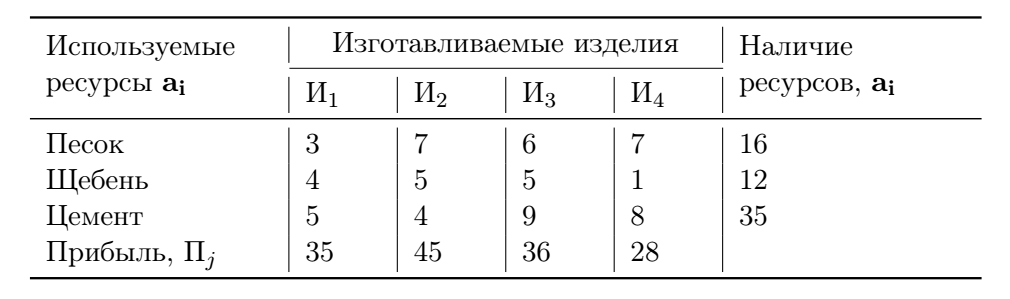
\includegraphics[scale=0.4]{JPG/ein.png}\\
Рисунок 1 -- Количество ресурсов находящихся в распоряжении завода\\
\end{center}
\newpage
\section{Функции}
\subsection{Решение уравнения}
Даны функции $f(x) = \sqrt{3}sin(x) + cos(x)$ и $g(x) = cos(2 \cdot x + \pi/3) - 1$ \\
\indent Задача решения уравнения $f(x) = g(x)$ эквивалентна нахождению корней уравнения $h(x) = f(x) - g(x)$:\\
$$y = \sqrt{3}sin(x) + cos(x) - cos(2 \cdot x + pi/3) + 1$$ \\
\indent Для того чтобы понять характер данного уравнения, построим график его функции (рисунок 2):\\
$function y = h(x)$ \\
$y = sqrt(3) * sin(x) + cos(x) - cos(2*x + \%pi/3) + 1$ \\
$endfunction$ \\
$plot(0:0.01:2*\%pi,h)$ \\
\begin{center} 
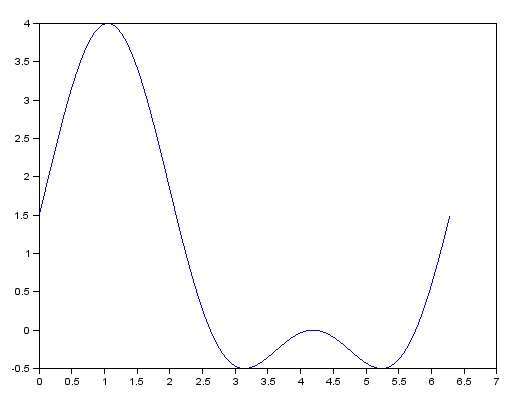
\includegraphics[scale=0.8]{JPG/zwei.jpg}\\
Рисунок 2 -- График функции $h(x)$\\
\end{center}
\indent Исходя из вида данного графика, можно сказать, что уравнение имеет от 2-ух до 4-ёх корней. Для получения данных корней применим функцию $fsolve$ задав вектор начальныч приближеных значений решения уравнения $x0$ (на основе построенного графика в точках $x0_1$ = 3, $x0_2$ = 4.2, $x0_3$ = 4.3, $x0_4$ = 5.5) получим вектор решений заданного уравнения $x$. $v$ -- вектор значений функции в точках $x$. \\
\indent Находим корни уравнения: \\
$deff('y=h(x)','y=sqrt(3)*sin(x)+cos(x)-cos(2*x+\%pi/3)+1')$ \\
$x0=[3,4.2,4.3,5.5]$; \\
$[x,v]=fsolve(x0,h)$ \\
 $v$  = \\
-2.220D-16 \quad 0. \quad 0. \quad 7.772D-16 \\
 $x$  = \\
   2.6179939 \quad 4.1887902 \quad 4.1887902 \quad 5.759586 \\
\indent Уранение имеет 3 корня: $x_1$ = 2.6179939, $x_2$ = 4.1887902 и $x_3$ = 5.759586. 
\indent Вследствие того, что решенное уравнение является тригонометрическим, можно предположить о кратности полученных решений числу $\pi$:\\
$x/\%pi$\\
 ans  =\\
   0.8333333 \quad 1.3333333 \quad 1.3333333 \quad 1.8333333\\
\indent Домножим данные решения на 3:\\
$3*x/\%pi$ \\
 ans  = \\
   2.5 \quad 4. \quad 4. \quad 5.5\\
\indent Полученые корни запишем в тригонометрической форме:\\
\begin{center}
$x_1 = \frac{5}{6}\pi + 2n\pi, n \in Z$\\
$x_2 = \frac{8}{6}\pi + 2n\pi, n \in Z$\\
$x_3 = \frac{11}{6}\pi + 2n\pi, n \in Z$\\
\end{center}
\subsection{Исследование функции.}
\indent Исследование функции  $h(x) = f(x) - g(x)$ на промежутке $[0;\frac{5}{6}\pi]$.\\
Исследование производных функции произведём с помощью Reduce-algebra.\\
\indent Найдём значение функции $f(x)$ в точках $x$=0 и $x=\frac{5}{6}\pi$ с помощью оператора подстановки $sub$: $sub(exp,f)=g$, где $g$-результат, полученный при подстановке списка алгебраических выражений $exp$ в функцию $f$. Упростим функцию $f(x) = \sqrt{3}sin(x) + cos(x) - cos(2 \cdot x + \pi/3) + 1$ перед вычислениями, получив $f(x) = 2sin(x+\pi/6)*(1+sin(x+\pi/6))$.\\
$h(x):=2sin(x+pi/6)*(1+sin(x+pi/6))$;\\
$sub(x=0,h1) = \frac{3}{2}$;\\
$sub(x=5pi/6,h2) = 0$;\\
\indent Найдём первую и вторую производную с помощью оператора $df$: $df(f,x,n) = dif$, где $dif$ – аналитическая форма производной $n$-го порядка для функции $f$ по переменной $x$.\\
$dh1:=df(h,x,h1)$;\\
$dh2:=df(h,x,h2)$;\\
\indent Построим графики первой (рисунок 3) и второй (рисунок 4) производной:\\
$plot(dh1,x=(0..5pi/6))$;\\
$plot(dh2,x=(0..5pi/6))$;\\
\indent Далее, используя математический пакет Scilab, основываясь на виде графиков первой и второй производной, найдём нули первой и второй производной, используя оператор $num\_solve$: $num\_solve(f,x = const) = f0$, где $f0$ – ноль функции $f$, найденный численно при начальной точке работы алгоритма $x = const.$\\
\begin{center}
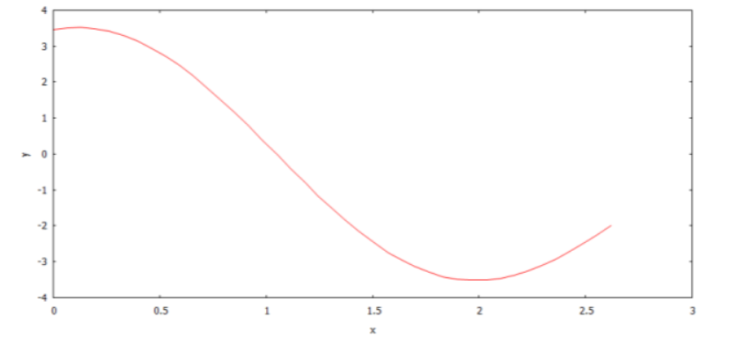
\includegraphics[scale=0.8]{JPG/drei.png}\\
Рисунок 3 -- График первой производной\\
\end{center}
\newpage
\indent Проведя необходимые вычисления, о функции, в исследуемом промежутке, можно сказать следующее:\\
\indent 1) Функция возрастает на промежутке $(0,\frac{\pi}{3})$;\\
\indent 2) Функция убывает на промежутке $(\frac{\pi}{3},\frac{5}{6}\pi)$;\\
\indent 3) Имеет максимум в точке $x$ = $\frac{\pi}{3}$;\\
\indent 4) Имеет минимум в точке $x = \frac{5}{6}\pi$;\\
\indent 5) Точки перегиба функции $x = 0.111$ и $x = 1.193$;\\
\indent 6) Выпукла вверх на промежутках (0,0.111) и (1.193,$\frac{5}{6}\pi)$;\\
\indent 7) Выпукла вниз на промежутке (0.111,1.193);\\
\begin{center}
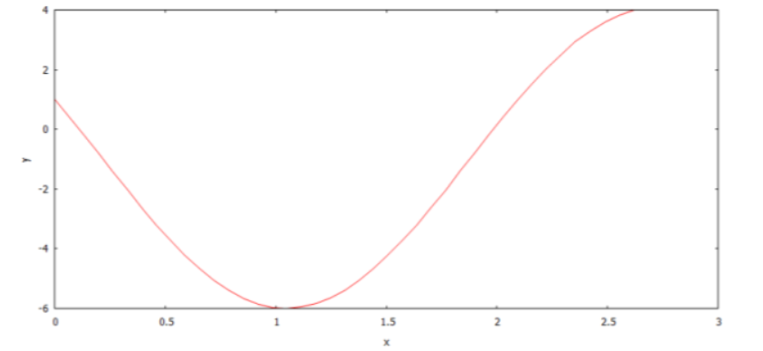
\includegraphics[scale=0.8]{JPG/vier.png}\\
Рисунок 4 -- График второй производной\\
\end{center}
\newpage
\section{Сплайны}\\
\subsection{Нахождение коэффициентов кубического сплайна}\\
\indent Для нахождения коэффициентов кубического сплайна представленных в векторах $V_x$ = [0,1.25,2.0,2.625,4.25] и $V_y$ = [3.0,2.925,3.75,3.42,4.444] решим уравнение $A_i \cdot Y_i^{-1} = C_f_i$:\\
\indent $i = 1:n$, где $n$ -- число столбцов вектора $V_x$, приусловии, что $V_x$ -- вектор-строка;\\
\indent $A_i$ = 
\begin{pmatrix}
1 & x_i & x_i^2 & x_i^3\\
1 & x_{i+1} & x_{i+1}^2 & x_{i+1}^3\\
0 & 1 & 2x_i & 3x_i^2\\
0 & 1 & 2x_{i+1} & 3x_{i+1}^2
\end{pmatrix},\\
где $x$ -- Узлы интерполяции;\\
\indent $Y_i$ = 
\begin{pmatrix}
y_i\\
y_{i+1}\\
d_i\\
d_{i+1}
\end{pmatrix},\\
где $y_i$ -- значение функции в узлах интерполяции,$d_i$ значение производной в углах интерполяции;\\
\indent $C_f_i$ - коэффициенты $i$-го кубического сплайна.\\
\noindent $x$ = [0,1.25,2.0,2.625,4.25]; \\
$y$ = [3.0,2.925,3.75,3.42,4.444]; \\
$d = splin(x,y)$; \\
$n = length(x)-1$; \\
$for i=1:4$ \\
    $a = x(i)$; \\
    $b = x(i+1)$; \\
    $cfs(:,i)$ = $[1,a,a^2,a^3; 1,b,b^2,b^3; 0,1,2*a,3*a^2; 0,1,2*b,3*b^2]$ / $[y(i);y(i+1);d(i);d(i++1)]$\\
$end$\\
$cfs$ =
  \begin{pmatrix}
3. & 3. & -10.113334 & -10.113334\\
- 2.9084975 & - 2.9084975 & 16.761504 & 16.761504\\
3.3405467 & 3.3405467 & -6.4944538 & -6.4944538\\
-0.849399 & -0.849399 & 0.7897678 & 0.7897678
\end{pmatrix}\\
\indent Первые два уравнения $1,a,a^2,a^3$; $1,b,b^2,b^3$ связывают значения многочлена с $y$-значениями; остальные два $0,1,2 \cdot a,3 \cdot a^2$; $0,1,2 \cdot b,3 \cdot b^2$ делают то же самое для своей производной. (Формулы являются просто производными от степени х). \\
Построим график функции $f(x)$ (рисунок 5) на основе полученных данных: \\
$for i$ = 1:4\\
    $t = linspace(x(i),x(i+1))$; \\
    $plot(t,cfs(:,i)'*[ones(t); t; t.^{\wedge}2; t.^{\wedge}3])$ \\
$end$ \\
\begin{center}
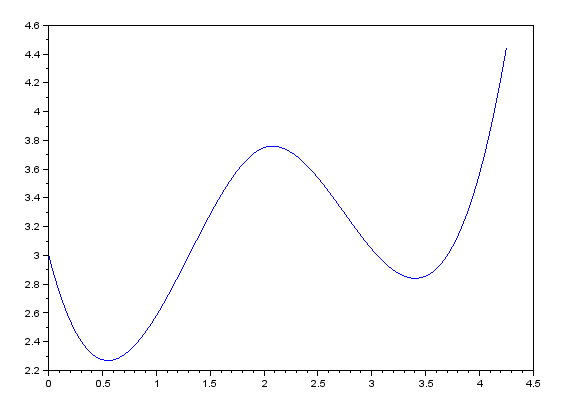
\includegraphics[scale=0.8]{JPG/funf.png}\\
Рисунок 5 -- График функции $f(x)$\\
\end{center}\\
\indent Найдем значение функции в точке $X$=1.8:\\
$x$ = [0,1.25,2.0,2.625,4.25]; \\
$y$ = [3.0,2.925,3.75,3.42,4.444];
$d = splin(x,y)$;
$X$=[1.8];\\
$Y=interp(X,x,y,d)$\\
$Y$  = 3.634381\\
\subsection{Встороенные функции Spline}
Графическое изображение результатов интерполяции исходных данных с использованием функций:\\
\indent -- $splin(x,y,"natural")$ -- кубический сплайн вычисляется при значениях второй производной начального $f''(x_1)$ и конечного $f''(x_n)$ значений равных нулю;\\
\indent -- $splin(x,y,"clamped")$ -- в этом случае кубический сплайн вычисляется с использованием производных в конце интервала, которые задаются в качестве последнего аргумента;\\
\indent -- $splin(x,y,"not\_a\_knot"),$ -- это случай по умолчанию, кубический сплайн вычисляется с учетом $n$ точек $x_1$,...,$x_n$;\\
\indent -- $splin(x,y,"fast")$ -- расчет сплайна происходит на основе обычной интерполяции кубическим полиномом;\\
\indent -- $splin(x,y,"monotone")$ -- в этом случае подсплайн вычисляется с использованием локальной схемы для точек, которая является монотонной в каждом интервале;\\
\indent -- $interp(xx,x,y,d)$ -- интерполяция полинома в точке $xx$, т.е. находится значение функции в этой точке,\\
осуществляется следующим способом: задаются известные точки графика функции ($x$ и $y$) и промежуток построения графика ($t$). Далее задаётся параметр $d$, соответствующий одной из функций и значения интерполяционного полинома ($ptd$) в точке ($t$): \\
$x$ = [0,1.25,2.0,2.625,4.25];\\
$y$ = [3.0,2.925,3.75,3.42,4.444];\\
$t$ = 0:0.01:4.445;\\
$d$ = $splin(x,y,"parametr")$\\
$ptd = interp(t,x,y,d)$\\
$plot2d(t,ptd)$\\
\indent На рисунке 6, 7 и 8 представлено графическое изображение результатов интерполяции с помощью функций $"natural"$, $"clamped"$ и $"not\_a\_knot"$ соответственно:\\
\begin{center}
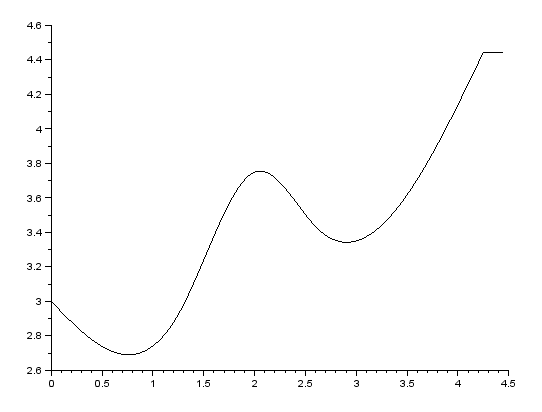
\includegraphics[scale=0.65]{JPG/nat.png}\\
Рисунок 6 -- Интерполянт $"natural"$\\
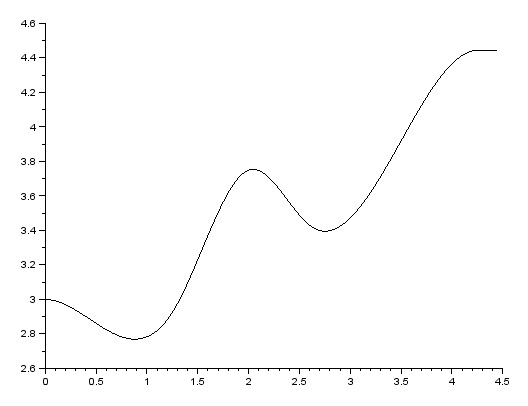
\includegraphics[scale=0.65]{JPG/clm.png}\\
Рисунок 7 -- Интерполянт $"clamped"$\\
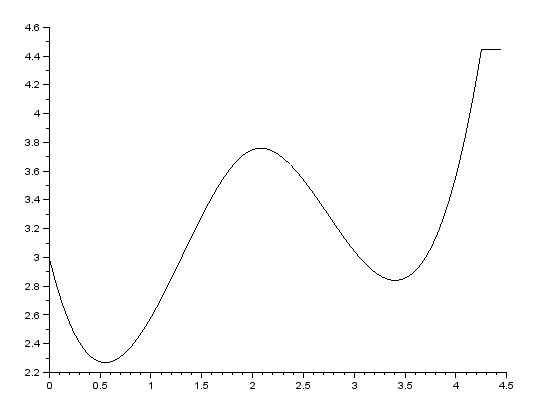
\includegraphics[scale=0.65]{JPG/not.png}\\
Рисунок 8 -- Интерполянт $"not\_a\_knot"$\\
\end{center}\\
\indent На рисунке 9 и 10 представлено графическое изображение результатов интерполяции с помощью функций $"fast"$ и $"monotone"$ соответственно:\\
\begin{center}
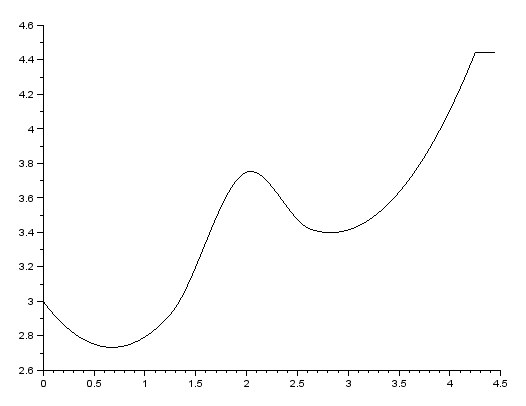
\includegraphics[scale=0.65]{JPG/fst.png}\\
Рисунок 9 -- Интерполянт $"fast"$\\
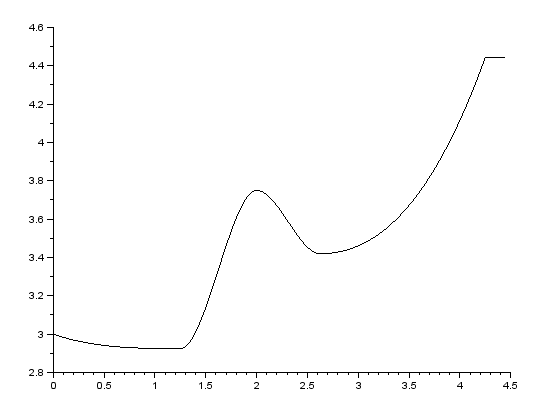
\includegraphics[scale=0.65]{JPG/mnt.png}\\
Рисунок 10 -- Интерполянт $"monotone"$\\
\end{center}\\
\newpage
\section{Оптимальное распределение неоднородных ресурсов}
\indent Пусть матрица $A$ размерности $mxn$ - количество сырья имеющегося в распоряжении завода железобетонных изделий, где $m$ - виды сырья (песок, щебень, цемент) и продукция $n$ видов. Вектора $b$ и $c$ - количество ресурсов на заводе и прибыль $с$ единицы изделия соответственно. $ci$ - вектор размерности $n$ содержащий нижнюю границу переменных ($ci_j > x_j$), $cs$ - вектор длиной $n$, содержащий верхнюю границу переменных ($cs_j > x_j$).\\
Для решения данной задачи воспользуемся функцией $linpro$. Функция $linpro$ возвращает массив неизвестных $x$, минимальное значение функции $f$ и массив множителей Лагранжа $kl$.\\
$c$ = [35;45;36;28];\\
$A$ = [3 7 6 7; 4 5 5 1; 5 4 9 8];\\
$b$ = [16;12;35];\\
$ci$ = [0;0;0;0];\\
$cs$ = [];\\
$[x,kl,f]=linpro(-c,A,b,ci,cs)$\\
$f$  =\\
- 126.56 \\
$x$  =\\
2.72\\
0.\\
0.\\
1.12\\
\indent В результате, для получения наибольшей прибыли f = 126.56, необходимо произвести 2.72 ед. продукции первого и 1.12 ед. продукции второго вида.\\
\newpage
\section{Вывод}\\
В результате выполнения курсовой работы с помощью математических пакетов Scilab и Reduce-algebra была решена и исследована функция $y = \sqrt{3}sin(x) + cos(x) - cos(2 \cdot x + pi/3) + 1$. Найдены коэффициенты кубического сплайна представленного в векторах $V_x$= [0,1.25,2.0,2.625,4.25] и $V_y$= [3.0,2.925,3.75,3.42,4.444], построен график сплайна на основе найденных коэффициентов и с помощью встроенных функций математического пакета Scilab. Была решена задача оптимального распределения имеющихся неоднородных ресурсов, условного предприятия для получения максимальной прибыли.
\newpage
\section{Список литературы}\\
\indent 1. Методические указания к курсовой работе по дисциплине "Информатика". М.П. Белов, А.К. Пожидаев, А.Н. Прокшин. Санкт-Петербургский государственный электротехнический университет "ЛЭТИ.\\
\indent 2.Алексеев Е. Р. Scilab: Решение инженерных и математических задач / Е. Р. Алексеев, О. В. Чеснокова, Е. А. Рудченко. М. : ALT Linux ; БИНОМ. Лаборатория знаний, 2008. 260 с.\\
\indent 3. КУБИЧЕСКИЕ СПЛАЙНЫ -- http://sernam.ru/book$_$mm3d.php?id=87\\
\indent 4. Интерполяция кубическими сплайнами -- http://www.machinelearning.ru\\/wiki/index.php?title=\%D0\%98\%D0\%BD\%D1\%82\%D0\%B5\%D1\%80\%D0\%BF\%D0\\\%BE\%D0\%BB\%D1\%8F\%D1\%86\%D0\%B8\%D1\%8F\_\%D0\%BA\%D1\%83\%D0\%B1\%\\D0\%B8\%D1\%87\%D0\%B5\%D1\%81\%D0\%BA\%D0\%B8\%D0\%BC\%D0\%B8\_\%D1\%81\\\%D0\%BF\%D0\%BB\%D0\%B0\%D0\%B9\%D0\%BD\%D0\%B0\%D0\%BC\%D0\%B8\\
\indent 5. Решение задач оптимизации средствами scilab и excel -- 
http://asu.ugatu.\\ac.ru/library/105/metodichkamatekonom.pdf\\
\indent 6. Создание графических интерфейсов и решение задач оптимизации средствами Scilab -- https://sites.google.com/site/resfizzs/praktika/resenie-zadac-linejno-\\go-programmirovania\\

\end{document}
